\section[bdt]{Boosted Decision Trees / Ensemble Methods}

\begin{frame}
    \frametitle{Idea}
    \begin{center}
      \textbf{Average many simple models to obtain a robust complex model}
      \begin{align*}
        F\left( \vec{x} \right) &= \sum_m \gamma_m f_m(\vec{x})
      \end{align*}
    \end{center}
\end{frame}

\begin{frame}
    \frametitle{Boosting}
    \begin{center}
      \begin{align*}
        f_m\left( \vec{x} \right) &= f_{m-1} + \mathrm{arg} \min_f \sum_i^N L \left(y_i, f_{m-1} (\vec{x}_i) - f(\vec{x}_i) \right)
      \end{align*}
      \begin{columns}
        \column{0.35\textwidth}
        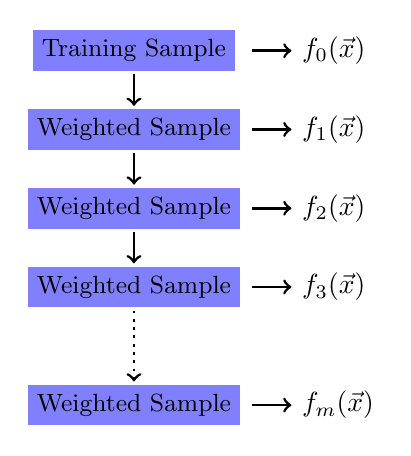
\begin{tikzpicture}
          \node[rectangle,fill=blue!50] at (0,0) {\small{Training Sample}};
          \node[rectangle,fill=blue!50] at (0,-1) {\small{Weighted Sample}};
          \node[rectangle,fill=blue!50] at (0,-2) {\small{Weighted Sample}};
          \node[rectangle,fill=blue!50] at (0,-3) {\small{Weighted Sample}};
          \node[rectangle,fill=blue!50] at (0,-4.5) {\small{Weighted Sample}};
          \draw[->,line width=1pt,Black] (1.5,0) -> (2,0) node[right] {$f_{0}(\vec{x})$};
          \draw[->,line width=1pt,Black] (1.5,-1) -> (2,-1) node[right] {$f_{1}(\vec{x})$};
          \draw[->,line width=1pt,Black] (1.5,-2) -> (2,-2) node[right] {$f_{2}(\vec{x})$};
          \draw[->,line width=1pt,Black] (1.5,-3) -> (2,-3) node[right] {$f_{3}(\vec{x})$};
          \draw[->,line width=1pt,Black] (1.5,-4.5) -> (2,-4.5) node[right] {$f_{m}(\vec{x})$};
          \draw[->,line width=1pt,Black] (0,-0.3) -> (0,-0.7);
          \draw[->,line width=1pt,Black] (0,-1.3) -> (0,-1.7);
          \draw[->,line width=1pt,Black] (0,-2.3) -> (0,-2.7);
          \draw[->,line width=1pt,Black,dotted] (0,-3.3) -> (0,-4.2);
        \end{tikzpicture}

        \column{0.65\textwidth}
        \begin{itemize}
          \item Reweight events w.r.t current prediction
          \item Individual classifiers are simple; in order to avoid overfitting (weak-learners)
          \item Focus on events near the optimal separation hyper-plane
          \item Loss function $L$ is crucial
            \begin{itemize}
              \item Least square $\rightarrow$ Regression
              \item Binomial deviance $\rightarrow$ GradientBoost classification
              \item Exponential loss $\rightarrow$ AdaBoost classification
            \end{itemize}
        \end{itemize}
      \end{columns}

    \end{center}
\end{frame}


\begin{frame}
    \frametitle{Bagging}
    \begin{center}
      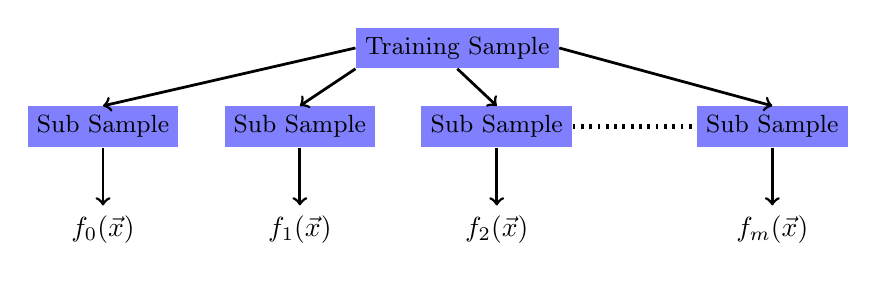
\begin{tikzpicture}
        \node[rectangle,fill=blue!50] (initial) at (0,1) {\small{Training Sample}};
        \node[rectangle,fill=blue!50] (first) at (-4.5,0) {\small{Sub Sample}};
        \node[rectangle,fill=blue!50] (second) at (-2,0) {\small{Sub Sample}};
        \node[rectangle,fill=blue!50] (third) at (0.5,0) {\small{Sub Sample}};
        \node[rectangle,fill=blue!50] (fourth) at (4,0) {\small{Sub Sample}};
        \draw[->,line width=1pt,Black] (first.south) -> (-4.5,-1) node[below] {$f_{0}(\vec{x})$};
        \draw[->,line width=1pt,Black] (second.south) -> (-2,-1) node[below] {$f_{1}(\vec{x})$};
        \draw[->,line width=1pt,Black] (third.south) -> (0.5,-1) node[below] {$f_{2}(\vec{x})$};
        \draw[->,line width=1pt,Black] (fourth.south) -> (4,-1) node[below] {$f_{m}(\vec{x})$};
        \draw[-,line width=1pt,Black,dotted, ultra thick] (third.east) -> (fourth.west);
        \draw[->,line width=1pt,Black] (initial.west) -> (first.north);
        \draw[->,line width=1pt,Black] (initial.south west) -> (second.north);
        \draw[->,line width=1pt,Black] (initial.south) -> (third.north);
        \draw[->,line width=1pt,Black] (initial.east) -> (fourth.north);
      \end{tikzpicture}

      \begin{itemize}
        \item Bagging -- Use only a fraction of events / features per classifier
        \item Robustness against statistical fluctuations in the data
        \item Embarrassingly parallel
        \item Sampling method is crucial:
          \begin{itemize}
            \item Draw random events with replacements $\rightarrow$ Bagging
            \item Draw random events without replacement $\rightarrow$ Pasting
            \item Draw random features $\rightarrow$ Random Subspaces
          \end{itemize}
      \end{itemize}

    \end{center}
\end{frame}

\begin{frame}
    \frametitle{Stochastic Boosted Decision Trees}
    \begin{center}
      \begin{itemize}
        \item Good out-of-the-box performance
        \item Robust against over-fitting
        \item Supports classification and regression
        \item Widely used in HEP
      \end{itemize}
      \begin{tikzpicture}
          \node[anchor=south west,inner sep=0] (image) at (0,0) {\includegraphics[width=0.6\textwidth]{forest_classifier.png}};
      \end{tikzpicture}
    \end{center}
\end{frame}

\begin{frame}
    \frametitle{Example Classifier Quality}
    \begin{center}
      \begin{tikzpicture}
          \node[anchor=south west,inner sep=0] (image) at (0,0) {\includegraphics[width=\textwidth]{forest_roc.png}};
      \end{tikzpicture}
    \end{center}
\end{frame}

\begin{frame}
    \frametitle{Further Ensemble Methods}
    \begin{center}
      \textbf{Categorization}
      \begin{itemize}
        \item Divide feature-space into sub-spaces
        \item Different behavior of the data in the chosen subspaces
        \item e.g. train separate classifiers for Barrel and Endcap
      \end{itemize}


      \begin{tikzpicture}
          \node[anchor=south west,inner sep=0] (image) at (0,0) {\includegraphics[width=0.4\textwidth]{belle2_detector.png}};
      \end{tikzpicture}


      \textbf{Combination}
      \begin{itemize}
        \item Combine different classifiers
        \item Different regularization methods learn different aspects of the data
        \item e.g. combine neural network, BDT and SVM
      \end{itemize}
    \end{center}
\end{frame}
